%% thesis.tex 2014/04/11
%
% Based on sample files of unknown authorship.
%
% The Current Maintainer of this work is Paul Vojta.

\documentclass{ucbthesis}

\usepackage[american]{babel}
\usepackage{csquotes}
\usepackage[backend=biber, style=apa]{biblatex}
\DeclareLanguageMapping{american}{american-apa}
\bibliography{../../Documents/References/references.bib}

\usepackage{amsmath}


% To compile this file, run "latex thesis", then "biber thesis"
% (or "bibtex thesis", if the output from latex asks for that instead),
% and then "latex thesis" (without the quotes in each case).

% Double spacing, if you want it.  Do not use for the final copy.
% \def\dsp{\def\baselinestretch{2.0}\large\normalsize}
% \dsp

% If the Grad. Division insists that the first paragraph of a section
% be indented (like the others), then include this line:
% \usepackage{indentfirst}

\newtheorem{theorem}{Jibberish}

\hyphenation{mar-gin-al-ia}
\hyphenation{bra-va-do}

\begin{document}

% Declarations for Front Matter

\title{Bayesian and frequentist cross-validation methods for clustered and cross-clustered data}
\author{Daniel C. Furr}
\degreesemester{Spring}
\degreeyear{1995}
\degree{Doctor of Philosophy}
\chair{Professor Sophia Rabe-Hesketh}
\othermembers{Professor Alan Hubbard \\
              Assistant Professor Zacahary Pardos}
\numberofmembers{3}
\field{Education}
\campus{Berkeley}


\maketitle
% Delete (or comment out) the \approvalpage line for the final version.
\approvalpage
\copyrightpage

\include{abstract}

\begin{frontmatter}

\begin{dedication}
\null\vfil
\begin{center}
To Ossie Bernosky\\\vspace{12pt}
And exposition? Of go. No upstairs do fingering. Or obstructive, or purposeful.
In the glitter. For so talented. Which is confines cocoa accomplished.
Masterpiece as devoted. My primal the narcotic. For cine? To by recollection
bleeding. That calf are infant. In clause. Be a popularly. A as midnight
transcript alike. Washable an acre. To canned, silence in foreign.
\end{center}
\vfil\null
\end{dedication}

% You can delete the \clearpage lines if you don't want these to start on
% separate pages.

\tableofcontents
\clearpage
\listoffigures
\clearpage
\listoftables

\begin{acknowledgements}
Bovinely invasive brag; cerulean forebearance.
Washable an acre. To canned, silence in foreign.
Be a popularly. A as midnight transcript alike.
To by recollection bleeding. That calf are infant. In clause.
Buckaroo loquaciousness?  Aristotelian!
Masterpiece as devoted. My primal the narcotic. For cine?
In the glitter. For so talented. Which is confines cocoa accomplished.
Or obstructive, or purposeful.
And exposition? Of go. No upstairs do fingering.

\end{acknowledgements}

\end{frontmatter}

\pagestyle{headings}

% (Optional) \part{First Part}

\newpage
\chapter{Cross-validation for cross-clustered data}
\documentclass[12pt, letterpaper]{article}
\usepackage[left=1.00in, right=1.00in, top=1.00in, bottom=1.00in]{geometry}
\usepackage{tikz}
  \usetikzlibrary{arrows.meta}
\usepackage{caption}
\usepackage{subcaption}
\usepackage{amsmath}

\usepackage[american]{babel}
\usepackage{csquotes}
\usepackage[backend=biber, style=apa]{biblatex}
\DeclareLanguageMapping{american}{american-apa}
\bibliography{../../../Documents/References/references.bib}

\title{Posterior predictive model checking and cross-validation for explanatory item response models}
\author{Daniel Furr}
\date{\today}




\begin{document}

% Tikz styles presets ----------------------------------------------------------

% Parameter and data nodes
\tikzstyle{p} = [circle, draw=black, fill=blue!10, thick,
                 inner sep=1pt, minimum size=8mm]
\tikzstyle{d} = [rectangle, draw=black, fill=blue!10, thick,
                 inner sep=1pt, minimum size=8mm]

% Replicate parameter and data nodes
\tikzstyle{pr} = [circle, draw=gray, fill=white, thick,
                  inner sep=1pt, minimum size=8mm]
\tikzstyle{dr} = [rectangle, draw=gray, fill=white, thick,
                  inner sep=1pt, minimum size=8mm]

% Arrow styles for model specification and for generating quantities
\tikzstyle{marrow} = [solid, -{Stealth[length=2mm]}, draw=black]
\tikzstyle{garrow} = [solid, -{Stealth[length=2mm]}, draw=gray]


% Invisisble node (for maintaining equal figure sizes_
\tikzstyle{i} = [circle, draw=none, fill=none, text=white]

% Box for PPCM part of model
\tikzstyle{ppmc}=[fill=red!10, draw=white]

% Boxes and labels to indicate clustering in models
\tikzstyle{items-box}    = [fill = none, draw = black!30!green]
\tikzstyle{items-node}   = [text = black!30!green, anchor = south east]
\tikzstyle{persons-box}  = [fill = none, draw = black!20!orange]
\tikzstyle{persons-node} = [text = black!20!orange, anchor = north west]

\newcommand{\comment}[1]{{\footnotesize[\textit{#1}]}}

\maketitle

\tableofcontents
\newpage
{\footnotesize }

\section{Introduction}

\section{A doubly explanatory item response model}

\subsection{General formulation}

A popular model for dichotomous item response data is the Rasch model \parencite{Rasch1960a}:
\begin{equation} \label{eq:base}
	\Pr ( y_{ip} | \theta_p, \delta_i) =
	\frac {\exp(\theta_p - \delta_i)^{y_{ip}}}
	{1 + \exp(\theta_p - \delta_i)}
,\end{equation}
where $y_{ip} = 1$ if person $p$ ($p = 1, \dotsc, P$) responded to item $i$ ($i = 1, \dotsc, I$) correctly and $y_{ip} = 0$ otherwise, $\theta_p$ is the ability parameter for person $p$, and $\delta_i$ is the difficulty parameter for item $i$. The individual instances of $\theta_p$ and $\delta_i$ may be collected into vectors $\theta$ and $\delta$, respectively. This is a ``descriptive'' item response model \parencite{Wilson2004}; it fully accounts for abilities and difficulties (assuming the appropriateness of the model), but does not offer insight into the the person or item predictors associated with abilities and difficulties.

The model in Equation~\ref{eq:base} may be expanded to a ``person explanatory'' model by decomposing $\theta_p$ as
\begin{equation} \label{eq:theta}
	\theta_p = w_p' \gamma + \zeta_p
,\end{equation}
where $w_p$ is a row from the design matrix of person-related covariates $W$, $\gamma$ is a vector of parameters, and $\zeta_p$ is the residual person abilities. The above may be interpreted as a latent regression of abilities on $W$. Henceforth, $\theta_p$ will be referred to as the composite ability, $w_p' \gamma$ the structured part of ability, and $\zeta_p$ the residual part. 

Similarly, decomposing $\delta_i$ as
\begin{equation} \label{eq:delta}
	\delta_i = x_i' \beta + \epsilon_i
\end{equation}
results in an ``item explanatory'' model, in which $x_i$ is a row from the design matrix of item-related covariates $X$, $\beta$ is a vector of parameters, and $\epsilon_i$ is the residual item difficulty. The above is then a latent regression of item difficulties on $X$. In parallel with the preceding terminology for ability, $\delta_i$ will be referred to as the composite difficulty, $x_i' \beta$ the structured part of difficulty, and $\epsilon_i$ the residual part. 

Equations~\ref{eq:base}, \ref{eq:theta}, and \ref{eq:delta} together form a ``doubly explanatory'' item response model, given that it incorporates covariates associated with both the person and item ``sides.'' Note that the model may still serve descriptive purpose as the composite abilities and difficulties remain a part of the model. The final step in formulating the model is to specify distributions for the residuals. Henceforth, normal distributions are assumed, 
\begin{equation}
	\zeta_p \sim N(0, \sigma^2)
\end{equation}
and
\begin{equation}
	\epsilon_i \sim N(0, \tau^2)
,\end{equation}
though other choices could be considered. The sides of the model are specified in directly parallel ways, and much of the discussion that follows will make use of this point.

The model is presented diagrammatically in Figure~\ref{fig:eirm-model}. In the diagram, the dependence on covariates $W$ and $X$ is suppressed. Parameters (loosely defined for the moment) are indicated by circles, and data are indicated by squares. The boxed regions indicate whether the parameters vary over persons, items or neither. The response data $y$ of course varies over both.

\begin{figure}[btp]
	\centering
	\centering
\begin{tikzpicture}[scale=.75, transform shape]

  \node [p]  (z)  at (0,10) {$\zeta$};
  \node [p]  (s)  at (2,10) {$\sigma$};

  \node [p]  (o)  at (0, 8) {$\theta$};
  \node [p]  (c)  at (2, 8) {$\gamma$};

  \node [d]  (y)  at (0, 6) {$y$};

  \node [p]  (d)  at (0, 4) {$\delta$};

  \node [p]  (e)  at (0, 2) {$\epsilon$};
  \node [p]  (b)  at (2, 4) {$\beta$};
  
  \node [p]  (t)  at (2, 2) {$\tau$};

  \draw [items-box] (-1, 0.75) rectangle (1.25, 7);
  \node [items-node] at (1.25, 0.75) {Items $i$};
  
  \draw [persons-box] (-1.25, 11.25) rectangle (1.00, 5);
  \node [persons-node] at (-1.25, 11.25) {Persons $p$};

  \foreach \from/\to in {s/z, c/o, z/o, o/y, d/y, b/d, t/e, e/d}
    \draw [marrow] (\from) -- (\to);

\end{tikzpicture}
	\caption{The full model. Circles represent parameters and squares represent data. Person covariates $W$ and item covariates $X$ are ommitted.}
	\label{fig:eirm-model}
\end{figure}


\subsection{Hierarchical Bayes modeling approach}

In Bayesian methodology, the joint posterior distribution for the parameters is factorized by way of Bayes theorem:
\begin{equation} \label{eq:bayes}
	p(\omega | y) \propto
	p(\omega)
	p(y | \omega)
,\end{equation}
which indicates that the joint posterior distribution proportional to the product of the joint prior distribution and the likelihood. In the above, $\omega$ is the set of model parameters. A taxonomy of parameters types is given below.
\begin{enumerate}
	\item \emph{Basic parameters}
	are the foundational parameters. They are plugged into the likelihood directly or affect it indirectly through intermediate parameters. Priors are specified for them.
	\begin{enumerate}
		\item \emph{Exchangeable basic parameters} 
		have hierarchical prior distributions. They are exchangeable draws from a distribution, the characteristics of which are determined by hyperparameters.
		\item \emph{Non-exchangeable basic parameters}
		have non-hierarchical (often non-informative) priors. They are not thought of as exchangeable or drawn from a distribution, except in the loose sense that there is a prior distribution.
	\end{enumerate}
	\item \emph{Intermediate parameters}
	are composites built from basic parameters. They are plugged into the likelihood in place of basic parameters.
	\item \emph{Hyperparameters}
	are parameters for the estimated distributions for exchangeable basic parameters. These are not plugged into the likelihood but rather determine the prior distributions for the exchangeable parameters.
\end{enumerate}
The doubly descriptive model has a likelihood (Equation~\ref{eq:base}) based on intermediate parameters $\theta$ and $\delta$, which are in turn built from basic parameters $\gamma$, $\zeta$, $\delta$, and $\epsilon$ (Equations~\ref{eq:theta} and \ref{eq:delta}). $\gamma$ and $\delta$ are non-exchangable basic parameters, while $\zeta$ and $\epsilon$ are exchangeable basic parameters whose priors depend on hyperparameters $\sigma$ and $\tau$, respectively.

The prior distribution in Equation~\ref{eq:bayes} may be rewritten as
\begin{equation} \label{eq:prior}
	p(\omega) =
	p(\gamma) p(\sigma)
	\left [ 
		\prod_{p=1}^P p(\zeta_p | \sigma) 
	\right ]
	p(\beta) p(\tau)
	\left [ 
		\prod_{i=1}^I p(\epsilon_i | \tau) 
	\right ]
,\end{equation}
assuming independent priors are specified, which is the usual case. No prior is included for $\theta$ and $\delta$ as they are wholly determined from the basic parameters. 
%The joint prior $p(\gamma, \beta, \tau, \sigma, \zeta, \epsilon)$ may be written as the product of individual priors if the priors are specified as independent, which is the usual case. 
The likelihood part of Equation~\ref{eq:bayes} may be rewritten in terms of basic parameters as
\begin{equation} \label{eq:bayes-likelihood-alt}
	p(y | \omega) =
	p(y | W, X, \gamma, \beta, \zeta, \epsilon) =
	\prod_{p=1}^P \prod_{i=1}^I 
	\Pr(y_{ip} | w_p, x_i, \zeta_p, \gamma, \epsilon_i, \beta)
\end{equation}
or in terms of intermediate parameters as
\begin{equation} \label{eq:bayes-likelihood}
	p(y | \omega) =
	p(y | \theta, \delta) =
	\prod_{p=1}^P \prod_{i=1}^I \Pr(y_{ip} | \theta_p, \delta_i)
.\end{equation}
Given that both the prior and the likelihood may be specified ignoring the intermediate parameters $\theta$ and $\delta$, it is clear that they are redundant. For many applications, however, they have useful interpretations. Further, the posterior distributions of $\theta$ and $\delta$ can be estimated easily using the posterior draws of the basic parameters.

%\comment{In practice (meaning in the results of Monte Carlo simulation of the proposed model), $\theta$ and $\delta$ are in the joint posterior. How should the notation reflect this fact? Link this topic to hierarchical centering.}

The posterior for a single parameter may be isolated by integrating the joint posterior over the other parameters. Let $D = \{ y, W, X \}$ represent the full data. Then,
\begin{equation}
	p(\sigma | D) = 
	\int \!\!\! \int \!\!\! \int \!\!\! \int \!\!\! \int
		p(\zeta, \gamma, \sigma, \epsilon, \beta, \tau | D) 
	~d \zeta d \gamma d \epsilon d \beta d \tau
\end{equation}
is the posterior for the standard deviation of the ability residuals. The mean and standard deviation of the marginal posterior for a parameter may be taken to represent a point estimate and standard error. Further, the joint posterior of a subset of parameters, $p(\beta, \zeta_p, \gamma, \epsilon_i | D)$ for example, likewise may be obtained by integrating out the other parameters. Despite the high-dimensional integral involved, these quantities are readily available from Monte Carlo simulation by simply ignoring the draws for the parameters to be integrated out, and so no special effort is required to obtain them.

Some alternative approaches to specifying the model bear mentioning. First, the model could equivalently be specified using hierarchical centering \parencite{gelfand1995efficient} by replacing the prior with
\begin{equation}
	p(\omega) =
	p(\gamma) p(\sigma)
	\left [ 
		\prod_{p=1}^P p(\theta_p | w_p, \gamma, \sigma)
	\right ]
	p(\beta) 	p(\tau)
	\left [ 
		\prod_{i=1}^I p(\delta_i | x_i, \beta, \tau) 
	\right ]
\end{equation}
where 
$p(\theta_p | w_p, \gamma, \sigma) = N(w_p \gamma, \sigma^2)$ and
$p(\delta_i | x_i, \beta, \tau)    = N(x_i \beta, \tau^2)$, 
respectively. The likelihood is specified as in Equation~\ref{eq:bayes-likelihood}, and $\zeta$ and $\epsilon$ are omitted altogether. Depending on the algorithm used for Monte Carlo simulation, this may improve the efficiency.
%With hierarchical models, the distinction between prior and likelihood is somewhat arbitrary. The priors for $\zeta_p$ and $\epsilon_i$ in Equation~\ref{eq:prior} may be considered part of the prior, in which case they may be thought of as ``empirical'' or ``estimated'' priors. Alternatively, they may be considered part of the likelihood, in which case Equation~\ref{eq:bayes-likelihood-alt} may be rewritten as
Second, a likelihood may be chosen that is marginal in regards to $\zeta$ and $\epsilon$:
\begin{equation} \label{eq:marginal-likelihood}
	p(y | \gamma, \beta, \sigma, \tau) =
	\iint
		\prod_{p=1}^P \prod_{i=1}^I 
		\Pr(y_{ip} | \zeta_p, \gamma, \epsilon_i, \beta)
		p(\zeta_p | \sigma)
		p(\epsilon_i | \tau)
	~d \zeta_p d \epsilon_i
.\end{equation}
The residuals $\zeta_p$ and $\epsilon_i$ are integrated out, and they are not included in the prior, which is simply $p(\gamma) p(\sigma) p(\beta) p(\tau)$.

%\comment{I find this discussion awkward. If both forms of the likelihood (marginal and conditional) get to live in the Bayes encampment, than discussion of frequentist and Bayes differences get muddled. This is especially true of the later discussion about what get called an estimate versus what is called a prediction. It's a prediction if it wasn't estimated, so inference for $\zeta_p$ is a prediction if the likelihood is marginal, whether or not we're standing with the frequentist and Bayesians. A smaller point: Do Bayesians fit models using marginal likelihoods? Does that work with Monte Carlo simulation? Or is it something that is occasionally mentioned but not a part of practice? If so (and I don't know), it may not belong in the Bayesian section. Or it could be that the distinction between types of likelihood is not so much a Frequenist vs Bayesian issue.}


\subsection{Frequentist modeling approach}

In the ``frequentist'' approach, only the non-exchangeable basic parameters ($\gamma$ and  $\beta$) and the hyperparameters ($\sigma$ and $\tau$) are treated as parameters to be estimated. The likelihood is specified as in Equation~\ref{eq:marginal-likelihood}, in which the probability of a response is marginal over the distributions for person and item residuals. Point estimates $\hat\gamma$, $\hat\sigma$, $\hat\beta$, and $\hat\tau$ are obtained by a process that maximizes this likelihood.

Within this framework, the exchangeable parameters $\zeta$ and $\epsilon$ are called latent variables or random effects because parameters cannot have distributions. Rather than obtain direct estimates for random effects, marginal maximum likelihood estimation obtains estimates for the parameters of their distributions, in this case, $\hat \sigma$ and $\hat\tau$. The non-exchangeable basic parameters $\gamma$ and $\beta$ are sometimes referred to as ``fixed-effects.''
\comment{``Can choose whether to treat $\zeta_p$ or $\epsilon_i$ as latent variables (random effects) or just consider their marginal likelihood, for example, to just get a covariance structure.'' Ref: Molenberghs and Verbeke. Hard to find because they wrote a million articles together.}

A model of this kind may be formulated in the generalized linear mixed model framework. The response variable, conditional on covariates and so-called random effects, is specified as arising from a Bernoulli distribution: 
\begin{equation}
	y_{ip} | w_p, x_i, \zeta_p, \epsilon_i \sim \mathrm{Bernoulli}(\pi_{ip})
.\end{equation}
Then the model may be written in terms of an inverse link function
\begin{equation}
	\pi_{ip} = 
	\Pr(y_{ip} = 1 | w_p, x_i, \zeta_p, \epsilon_i) =
	\mathrm{logit}^{-1}[\eta_{ip}]
\end{equation}
and a linear predictor
\begin{equation}
	\eta_{ip} =
	(w_p'\gamma + \zeta_p) -
	(x_i'\beta + \epsilon_i)
.\end{equation}
Because the random-effects $\zeta_p$ and $\epsilon_i$ are not nested, the model may be described as a crossed-mixed effects model. Such a model is difficult to estimate efficiently via marginal maximum likelihood because the integrals in Equation~\ref{eq:mml-likelihood} do not factorize as they do with nested random effects. The result is an $I \times P$ dimensional integral, though \textcite{rasbash1994efficient} describe a means of reducing this to an $I + 1$ dimensional integral.

%double integration over the latent distributions (see Equation~\ref{eq:mml-likelihood}). The Laplace approximation may be employed to make the math tractable, but this approach has known shortcomings \parencite{Joe2008}.

%Though not directly estimated, post-hoc estimates for $\hat\zeta_p$ and $\hat\epsilon_i$ may be obtained by finding the mean or mode of $p(\yp|\zeta_p) p(\zeta_p|\hat\sigma)$ or $p(\yi|\epsilon_i) p(\epsilon_i|\hat\tau)$, which are referred to as ``empirical Bayes'' estimates. Standard errors are available for these, though they are calculated as though the parameter estimates are known, rather than random, quantities.
%
%Also available only in post-analysis are estimates
%$\hat\theta_p = w_p' \hat\gamma + \hat\zeta_p$ and
%$\hat\delta_i = x_i' \hat\beta + \hat\epsilon_i$,
%where $\hat\zeta_p$ and $\hat\epsilon_i$ are empirical Bayes estimates. Standard errors are available for these quantities, though they also are calculated as if the parameter estimates are known quantities.


\subsection{Special cases}
\label{sec:special-cases}

Many dichotomous item response models are special cases of the doubly explanatory model that arise from restrictions placed on the composite abilities and difficulties. For example, the variant of the Rasch model \parencite{Rasch1960a} associated with marginal maximum likelihood estimation \parencite{bock1981marginal} can be written as
\begin{equation}
	\Pr ( y_{ip} | \theta_p, \delta_i) =
	\frac {\exp(\theta_p - \delta_i)^{y_{ip}}}
	{1 + \exp(\theta_p - \delta_i)}
\end{equation}
\begin{equation}
	\theta_p = \zeta_p
\end{equation}
\begin{equation}
	\delta_i = x_i' \beta
,\end{equation}
where $X$ is an $I \times I$ identity matrix ($I_I$) and $\beta$ is a vector of length $I$, such that $\delta_i = \beta_i$. In other words, $\theta_p$ is set equal to the ability residuals, and $\delta_i$ is set equal to the (unstructured) structural part.

In the Bayesian approach, the posterior for this Rasch model variant is given by
\begin{equation}
	p(\theta, \sigma, \delta | y) \propto
	\left [ 
		p(\delta) 	p(\sigma)
		\prod_{p=1}^P p(\theta_p | \sigma) 
	\right ]
	\left [ 
		\prod_{p=1}^P \prod_{i=1}^I 
		\Pr ( y_{ip} | \theta_p, \delta_i) 
	\right ]
,\end{equation}
in which the left hand bracketed quantity is the prior and and the right hand quantity is the likelihood. The marginal likelihood for the frequentist approach is
\begin{equation}
	p(y | \sigma, \delta) =
	\prod_{p=1}^P
	\int
		\prod_{i=1}^I 
		\Pr(y_{ip} | \theta_p, \delta_i)
		p(\theta_p | \sigma)
	~d \theta_p
.\end{equation}
The single dimensional integration is simpler than the $I \times P$ dimensional integral in Equation~\ref{eq:marginal-likelihood} and is normally approximated using adaptive quadrature.

\begin{table}
	\centering
	\begin{tabular}{lccc}
		\hline
		Model	& $\theta_p$ & $\delta_i$ & Notes \\ \hline
		MML Rasch
			& $\zeta_p$ & $x_i'\beta$ & $X = I_I$ \\ 
		JML Rasch
			& $w_p' \gamma$ & $x_i'\beta$ & $W = I_{P-1}$, $X = I_I$ \\ 
		Random item Rasch
			& $\zeta_p$ & $\epsilon_i$ &  \\ 
		Latent regression
			& $w_p' \gamma + \zeta_p$ & $x_i'\beta$ & $X = I_I$ \\ 
		Linear logistic test
			& $\zeta_p$ & $x_i'\beta$ &  \\ 
		Linear logistic test with error
			& $\zeta_p$ & $x_i'\beta + \epsilon_i$ &  \\ 
		Doubly explanatory
			& $w_p' \gamma + \zeta_p$ &  $x_i'\beta + \epsilon_i$ & \\
		\hline
	\end{tabular}
	\caption{Specification of several special cases.}
	\label{tab:special-cases}
\end{table}

Other special cases arise from different choices of restrictions placed on the composite abilities and difficulties, and these are summarized in Table~\ref{tab:special-cases}. The variant of the Rasch model associated with joint maximum likelihood estimation \parencite[e.g.,]{embretson2000item} includes only the structured parts of ability and difficulty with identity matrices for $W$ and $X$ (one difficulty or ability parameter must be constrained for identifiability). In contrast, the random item Rasch model \parencite[e.g.,]{DeBoeck2008} has only the residual parts for both sides (a model intercept must be added). The latent regression item response model \parencite{Mislevy1985, Adams1997b} includes the both parts of the composite ability and the structured part of item difficulty, where $X$ is an identity matrix. The linear logistic test model (LLTM) \parencite{Fischer1973}, has the residual part for ability and the structured part for difficulty. Its extension, the linear logistic test model with error (LLTM-E) \parencite[e.g.,]{mislevy1988exploiting, Janssen2004}, adds an item difficulty residual. 


\section{Estimated and predicted quantities}

Several quantities from the fitted model may be of interest. At the macro-level, $\gamma$ represents the effects of the person covariates, and $W \gamma$ together with $\sigma$ describes the conditional distribution for person abilities. Likewise, $\beta$ represents the effects of the item covariates, and $X \beta$ together with $\tau$ describes the conditional distribution for item difficulties. Depending on the choice of either a frequentist and Bayesian framework, the maximum likelihood estimates $\hat \gamma$ and $\hat \beta$ or posterior distributions $p(\gamma | D)$ and $p(\beta | D)$ will be obtained for these parameters.

For some applications, such as measurement ``per se'' and model assessment, the individual persons and items may be of interest. In this case, focus will be placed on $\theta$, $\delta$, $\zeta$, and $\epsilon$. The intermediate parameters $\theta$ and $\delta$ will be of interest for measurement per se, while the residuals $\zeta$ and $\epsilon$ will be useful for model assessment. These are within-sample quantities; that is, the estimation sample contains a person $p$ who is associated with $\zeta_p$ and $\theta_p$ and also an item $i$ that is associated with $\epsilon_i$ and $\delta_i$. 

There may be a (real or hypothetical) person $p'$ who is not represented in the estimation data. This out-of-sample person $p'$ has a covariate vector $w_{p'}$ and is associated with parameters $\tilde \zeta_{p'}$ and $\tilde \theta_{p'}$, none of which play a role in fitting the model. Likewise, an out-of-sample item $i'$ associated with $w_{p'}$, $\tilde \epsilon_{i'}$, and $\tilde \delta_{i'}$ may be envisioned.

Inferences for the within-sample quantities $\theta_p$, $\delta_i$, $\zeta_p$, and $\epsilon_i$ are called predictions in the frequentist framework because they are random quantities not directly estimated from the model. Such inferences are called estimates in a Bayesian setting because they are obtainable from the posterior. Inferences for the out-of-sample quantities $\tilde \theta_{p'}$, $\tilde \delta_{i'}$, $\tilde \zeta_{p'}$, and $\tilde \epsilon_{i'}$ and are considered predictions in either case.

Lastly, inferences may be made regarding new responses, which are always considered predictions. A new response may be conceived as arising from a within-sample person-item pair, indicated by $\tilde y_{ip}$. This is, in other words, simply the model-predicted response for a within-sample observation. Several possibilities exist for out-of-sample responses: $\tilde y_{i'p}$ represents a new response from a within-sample person to an out-of-sample item, $\tilde y_{ip'}$ represents a new response from an out-of-sample person to a within-sample item, and $\tilde y_{i'p'}$ represents a totally out-of-sample response. Predictions for out-of-sample responses are termed forecasting in a longitudinal setting.


\subsection{Inferences for within-sample persons and items}

If the doubly explanatory model is estimated using the Bayesian estimation approach outlined above, posterior distributions for both the composite abilities, $p(\theta_p | D)$, and residual abilities, $p(\zeta_p | D)$, will be available. Likewise, posteriors for the composite item difficulties, $p(\delta_i | D)$, and residual item difficulties, $p(\epsilon_i | D)$, will be available. 

The posterior predictive distribution \parencite{rubin1984bayesianly} for new a response $\tilde y_{ip}$ from a within-sample person-item pair, in terms of intermediate parameters, is
\begin{equation}
	p(\tilde y_{ip} | D) =
	\iint
		\Pr (\tilde y_{ip} | \theta_p, \delta_i)
		p(\theta_p, \delta_i | D)
	~d\theta_p d\delta_i
,\end{equation}
or equivalently, in terms of basic and hyperparameters is
\begin{equation} \label{eq:yrep-post}
	p(\tilde y_{ip} | D;  \zeta_p, \epsilon_i) =
	\iiiint
		\Pr (\tilde y_{ip} | \gamma, \zeta_p, \beta, \delta_i)
		p(\gamma, \zeta_p, \beta, \delta_i | D)
	~d\gamma d\zeta_p d\beta d\delta_i
.\end{equation}
This is depicted in Figure~\ref{subfig:ppmc-same-both}. On the left side is a graphical representation of the model, similar to the one shown earlier, and on the right side is a shaded region for out-of-sample predictions. The diagram makes clear that $\tilde y_{ip}$ will closely resemble $y_{ip}$ because both arise from the same $\theta_p$ and $\delta_i$, assuming the correctness of the model.

\begin{figure}[btp]
	\centering
	\begin{subfigure}[b]{.4\textwidth}
		\input{figs/ppmc-same-both.tex}
		\caption{Within-sample persons and items}
		\label{subfig:ppmc-same-both}
	\end{subfigure}
	~
	\begin{subfigure}[b]{.4\textwidth}
		\input{figs/ppmc-new-both.tex}
		\caption{Out-of-sample persons and items}
		\label{subfig:ppmc-new-both}
	\end{subfigure}
	~
	\begin{subfigure}[b]{.4\textwidth}
		\input{figs/ppmc-new-theta.tex}
		\caption{Out-of-sample persons, within-sample items}
		\label{subfig:ppmc-new-persons}
	\end{subfigure}
	~
	\begin{subfigure}[b]{.4\textwidth}
		\centering
\begin{tikzpicture}[scale=.75, transform shape]

  \filldraw [ppmc] (3.25, 1.25) rectangle (4.75, 10.75);
  \node [i]  at (0, 12) {~}; % Force some vertical space with invisible node.

  \node [p]  (z)  at (0,10) {$\zeta$};
  \node [p]  (s)  at (2,10) {$\sigma$};

  \node [p]  (o)  at (0, 8) {$\theta$};
  \node [p]  (c)  at (2, 8) {$\gamma$};

  \node [d]  (y)  at (0, 6) {$y$};
  \node [dr] (yr) at (4, 6) {$\tilde y$};

  \node [p]  (d)  at (0, 4) {$\delta$};
  \node [p]  (b)  at (2, 4) {$\beta$};
  \node [pr] (dr) at (4, 4) {$\tilde \delta$};

  \node [p]  (e)  at (0, 2) {$\epsilon$};
  \node [p]  (t)  at (2, 2) {$\tau$};
  \node [pr] (er) at (4, 2) {$\tilde \epsilon$};

  \foreach \from/\to in {s/z, c/o, z/o, o/y, d/y, b/d, t/e, e/d}
    \draw [marrow] (\from) -- (\to);

  \foreach \from/\to in {o/yr, t/er, er/dr, b/dr, dr/yr}
    \draw [garrow] (\from) -- (\to);

\end{tikzpicture}

		\caption{Within-sample persons, out-of-sample items}
		\label{subfig:ppmc-new-items}
	\end{subfigure}
	\caption{Diagrams for generating predictive distributions of various forms. Circles represent parameters and squares represent data. The shaded region indicates predictive quantities that are not involved in the estimation. Covariates $W$ and $X$ are omitted.}
	\label{fig:ppmc-models}
\end{figure}


\subsection{Inferences for out-of-sample persons and items}

The predictive distribution for the residual ability for an out-of-sample person is
\begin{equation} \label{eq:zeta-mixed}
	p(\tilde \zeta_{p'} | D) = 
	\int
		p(\tilde \zeta_{p'} | \sigma)
		p(\sigma | D)
	~d\sigma
,\end{equation}
where $\tilde \zeta_{p'}$ indicates the new residual. This is referred to as mixed predictive distribution \parencite{Gelman1996}, as $\tilde \zeta_{p'}$ is drawn from its prior and $\sigma$ is drawn from its posterior. The mixed predictive distribution for a new composite ability is denoted by $p(\tilde \theta_{p'} | D)$, which is a function of 
	$p(\gamma, \tilde \zeta_{p'} | D) = 
	\int p(\tilde \zeta_{p'} | \sigma) p(\gamma, \sigma | D) ~d \sigma$
and the new covariate vector $w_p'$.

Predictive distributions for out-of-sample items may be discussed in a manner parallel to out-of-sample persons. The mixed predictive distribution for a new item residual, $p(\tilde \epsilon_{i'} | D)$, is derived in a similar way as in Equation~\ref{eq:zeta-mixed}. The mixed predictive distribution for the composite difficulty for a new item is $p(\tilde \delta_{i'} | D)$, and this is a function of $p(\beta, \tilde \epsilon_{i'} | D)$ and $x_i$.

The predictive distribution for a new response arising from an out-of-sample person and out-of-sample item may be specified in terms of the composite abilities and difficulties:
\begin{equation}
	p(\tilde y_{i'p'} | D) =
	\iint
		\Pr (\tilde y_{i'p'} | \tilde \theta_{p'}, \tilde \delta_{i'})
		p(\tilde \theta_{p'}, \tilde \delta_{i'} | D)
	~d\tilde \theta_{p'} d \tilde \delta_{i'}
.\end{equation}
Alternatively, it may be specified in terms of the residual parts, structural parts, and covariates:
\begin{equation}
	p(\tilde y_{i'p'} | D) =
	\iiiint
		\Pr (\tilde y_{i'p'} | \gamma,\tilde \zeta_{p'}, \beta, 
			\tilde \epsilon_{i'}, w_p, x_i)
		p(\gamma, \tilde \zeta_{p'}, \beta, \tilde \epsilon_{i'} | D)
	~d\gamma d \tilde \zeta_{p'} d \beta d \tilde \epsilon_{i'}
,\end{equation}
where
\begin{equation}
	p(\gamma, \tilde \zeta_{p'}, \beta, \tilde \epsilon_{i'} | D) = 
	\iint
		p(\tilde \zeta_{p'} | \sigma)
		p(\tilde \epsilon_{i'} | \tau)
		 p(\gamma, \sigma, \beta, \tau | D)
	~d \sigma d \tau
.\end{equation}
Figure~\ref{subfig:ppmc-new-both} depicts how the predictive distribution for $\tilde y_{i'p'}$ is formed. Because $\tilde y_{i'p'}$ arises from $\tilde \theta_p$ and $\tilde \delta_i$, it will differ substantially from $y_{ip}$ unless $W \gamma$ and $X \beta$ are such that the estimated $\sigma$ and $\tau$ are near zero.


\subsection{Inferences for mixed within-sample and out-of-sample responses}

A new response could, for example, come from an within-sample person but an out-of-sample item. The predictive distribution for such a response,
\begin{equation}
	p(\tilde y_{i'p} | D) = 
	\iint
		\Pr (\tilde y_{i'p} | \theta_{p}, \tilde \delta_{i'})
		p(\theta_{p}, \tilde \delta_{i'} | D)
	~d \theta_{p} d \tilde \delta_{i'}
,\end{equation}
relies on the joint distribution comprised of the posterior for $\theta_{p}$ and the mixed predictive distribution for $\tilde \delta_{i'}$.
Alternatively, it may be specified in terms of the residual parts, structural parts, and covariates:
\begin{equation}
	p(\tilde y_{i'p} | D) =
	\iiiint
		\Pr (\tilde y_{i'p'} | \gamma,\zeta_{p}, \beta, \tilde \epsilon_{i'}, 
			w_p, x_i)
		p(\gamma, \zeta_{p}, \beta, \tilde \epsilon_{i'} | D)
	~d\gamma d \zeta_{p} d \beta d \tilde \epsilon_{i'}
,\end{equation}
where
\begin{equation}
	p(\gamma, \zeta_{p}, \beta, \tilde \epsilon_{i'} | D) = 
	\int
		p(\tilde \epsilon_{i'} | \tau)
		p(\gamma, \zeta_p, \beta, \tau | D)
	~d \tau
.\end{equation}
The prediction for $\tilde y_{i'p}$ is depicted in Figure~\ref{subfig:ppmc-new-items}. 

If instead the predictive distribution for a new response from a out-of-sample person but within-sample item is needed, then $p(\tilde y_{ip'} | D)$ may be derived based on a joint distribution comprised of the posterior for $\delta_{i}$ and the mixed predictive distribution for $\tilde \theta_{p'}$. This is depicted in Figure~\ref{subfig:ppmc-new-persons}.


\subsection{Inferences for special cases}

If a special case of the full model is fitted, such as any described in Section~\ref{sec:special-cases}, some predictive inferences may not be available. Specifically, a parameter must be exchangeable (that is, drawn from a distribution) in order to specify a predictive distribution for it. For example, with the Rasch model (either of the marginal or joint maximum likelihood formulations) predictive distributions for $\tilde \delta_{i'}$ and $\tilde y_{i'p}$ are unavailable due the restriction $\delta = X \beta$. 
\comment{I may decide this section isn't important.}

%With a simpler model, such as the Rasch model with exchangeable persons described in Section~\ref{sec:special-cases}, fewer variations are on prediction are available. For this model, posterior distributions are of course available for $\theta_p$ and $\delta_i$, and there is also the mixed predictive distribution $p(\tilde \theta_{p'} | \D)$. Given that $\delta_i$ is a non-exchangeable parameter in the Rasch model, there is no mixed predictive distribution for it. A new response must involve an existing item, but may arise from either an existing person, leading to the predictive distribution $p(\tilde y_{ip} | \D)$, or new person, leading to $p(\tilde y_{ip'} | \D)$.


\subsection{Frequentist prediction methods}

\section{Posterior predictive model checking}

\section{Cross-validation}


\printbibliography

\end{document}


\newpage
\chapter{Frequentist cross-validation with the doubly explanatory model}
\chaptermark{Frequentist cross-validation}
\documentclass[12pt, letterpaper]{article}
\usepackage[left=1.00in, right=1.00in, top=1.00in, bottom=1.00in]{geometry}
\usepackage{amsmath}
\usepackage{apacite}
\usepackage{graphicx}

\title{Chapter 2}
\author{Daniel C. Furr}
\date{\today}


\begin{document}

\newcommand{\genupsilonsq}{0.11}
\newcommand{\gentau}{\{0.00, 0.10, 0.30, 0.50\}}
\newcommand{\gentausq}{\{0.00, 0.01, 0.09, 0.25\}}
\newcommand{\genrsq}{\{1.00, 0.92, 0.55, 0.30\}}

\newcommand{\comment}[1]{{\footnotesize[\textit{#1}]}}

\maketitle

\tableofcontents
\newpage
{\footnotesize }


\section{Introduction}

%\begin{enumerate}
%	\item Conducting holdout cross-validation require a decision of what parts of model are exchangeable. Approximations also depend on this, though may not be obvious. Easy for non-clustered data. For clustered data, must decide whether clusters are exchangeable. In a model with likelihood that is marginal over clusters, it is implied that clusters are exchangeable.
%	\item Item response models generally have fixed part for items and random part for persons, reflecting an expectation that new data would have new people responding to the original items. CV ``over persons'' may be used to select person predictors.
%	\item Not appropriate for selecting predictors for item difficulty. Need CV ``over items''. LLTM marginal likelihood not appropriate. LLTME marginal likelihood is appropriate, though difficult.
%	\item This paper shows...
%\end{enumerate}

The use of cross-validation with clustered data requires a decision as to what aspects of the data are exchangeable, and so are resampled in new data, and what aspects persist. For item response data, in which responses are nested both within persons and items simultaneously, new data may consist of a new group of persons responding to the original items, which will be referred to as cross-validation ``over persons.'' Alternatively, new item response data may entail a new set of items presented to the original group of persons, which will be referred to as cross-validation ``over items.'' Other variations are possible, such as new data from both the same persons and items, an exact replication of the original data collection, or new data from both new persons and items.

The form of new data determines what inferences may be made using cross-validation. For example, cross-validation must be done over persons in order to select for person ability predictors in a latent regression Rasch model \cite{}. In other words, a new sample of persons are needed to assess the predictors for ability. Likewise, if the goal is to choose predictors for item difficulty in a linear logistic test model (LLTM) \cite{}, cross-validation must be performed over items.

The choice of model has strong implications regarding which aspects of the data are considered exchangeable, and hence would be resampled in cross-validation, and which are persistent. Specifically, the ``random effects'' are exchangeable, and the ``fixed effects'' are persistent. In general for item response models, person abilities (or their residuals) are modeled as random effects, while items are treated as fixed, implying that a repeat of the data collection would involve a new sample of persons responding to the same items.

In this chapter, the difference in efficacy of employing cross-validation over persons versus over items with LLTM is investigated. AIC, a single dataset approximation to cross-validation, is shown to correspond to cross-validation over persons, which is not effective for the selection of item predictors.


\section{Simulation and analysis methods}

\subsection{Data generation}

%Data are simulated for varying numbers of persons ($P$) and items ($I$) using the model described in Chapter~1. 
Data are simulated using the model described in Chapter~1. 
Specifically, the composite item difficulties are generated as
\begin{equation}
	\delta_i = x_{1i}\beta_1 + x_{2i}\beta_2 + x_{3i}\beta_3 + x_{4i}\beta_4 + x_{2i}x_{3i}\beta_5 + \epsilon_i
\end{equation}
\begin{equation}
	\epsilon_i \sim \mathrm{N}(0, \tau^2)
,\end{equation}
where $x_{1i} = 1$ is an intercept and $x_{2i}$, $x_{3i}$, and $x_{4i}$ are indicator variables which each equal 1 for half of the items and 0 for the remainder. Each possible combination of the indicators occurs an equal number of times, and the generating model includes one interaction, $x_{2i}x_{3i}$. Table~\ref{tab:X} provides the design matrix for item covariates. The rows of the design matrix are repeated to accommodate multiples of $I = 8n_p$.

% matrix: X file: figs/table_x.tex  23 Oct 2015 12:20:52
\begin{table}[htbp]
\caption{\label{tab:X} Items design matrix}\centering\medskip
\begin{tabular}{ccccc} \hline \hline
$x_1$ & $x_2$  & $x_3$  & $x_4$  \\  \hline 
1 & 0 & 0 & 0 \\  
1 & 0 & 0 & 1 \\  
1 & 0 & 1 & 0 \\  
1 & 0 & 1 & 1 \\  
1 & 1 & 0 & 0 \\  
1 & 1 & 0 & 1 \\  
1 & 1 & 1 & 0 \\  
1 & 1 & 1 & 1 \\  
\hline \hline \end{tabular}
\end{table}


The composite abilities are generated as
\begin{equation} \label{eq:theta}
	\theta_p = w_{1p}\gamma_1 + w_{2p}\gamma_2  + \zeta_p
\end{equation}
\begin{equation} \label{eq:zeta}
	\zeta_p \sim \mathrm{N}(0, \sigma^2)
,\end{equation}
where $w_{1p}$ and $w_{2p}$ are also crossed indicator variables. Table~\ref{tab:W} presents the design matrix for person covariates, the rows of which are repeated to accommodate the $P = 4n_i$ persons.

% matrix: W file: figs/table_w.tex  23 Oct 2015 12:20:52
\begin{table}[htbp]
\caption{\label{tab:W} Persons design matrix}\centering\medskip
\begin{tabular}{cc} \hline \hline
$w_1$  & $w_2$  \\  \hline 
0 & 0 \\  
0 & 1 \\  
1 & 0 \\  
1 & 1 \\  
\hline \hline \end{tabular}
\end{table}


A key feature of the generated datasets (and data of this type more generally) is the extent to which the item covariates account for the composite item difficulties. To this end, let $\upsilon^2 = \mathrm{var}(x'\mathbf{\beta})$ represent the variance of the structural part of item difficulty. Because of the item design, $\upsilon^2$ does not vary between simulated datasets, even if they have differing numbers of items (in multiples of eight). The total item variance is $\upsilon^2 + \tau^2$. Then
\begin{equation}
R^2 = \frac{\upsilon^2}{\upsilon^2 + \tau^2}
\end{equation}
represents the proportion of item variance accounted for by the item predictors. 

The generating values for the structural part of item difficulties are $\beta = \{ -.5, .5, .5, .5, -.5 \}$ in all simulation conditions, and so $\upsilon^2 = \genupsilonsq$. Figure~\ref{fig:rsq-vs-tau} displays $R^2$ as a function of $\tau$ with $\upsilon^2$ fixed to this value. The points indicate the generating values of $\tau$, which are $\tau \in \{\gentau\}$ (or equivalently,  $\tau^2 \in \{\gentausq\}$). These values yield $R^2 \in \{\rsq\}$. On the person side, the generating values are fixed across conditions, with $\gamma = \{ .5, .5 \}$ and $\sigma = 1$. 
%The numbers of persons and items vary: $I \in \{32, 128\}$ and $P \in \{300, 1000\}$.

\begin{figure}[tbp]
	\centering
	\includegraphics{chapter_2/figs/rsq_vs_tau.pdf}
	\caption{Proportion of total item variance explained by the item covariates ($R^2$) versus residual item standard deviation ($\tau$) in the simulated datasets. The points indicate generating values of $\tau \in \{\gentau\}$.}
	\label{fig:rsq-vs-tau}
\end{figure}

%In summary, three factors are varied between simulation conditions in a crossed design: $\tau$ (and by extention, $R^2$), $I$, and $P$. 
%All other elements are fixed across conditions. 
In summary, the same generating values and design matrices are used across all simulation conditions.
In the first simulation, generating values of $\tau$ are varied. In the second, the number of items are varied.
To employ cross-validation, multiple datasets are simulated within each replication: the ``test'' dataset, a ``training'' dataset representing a sample with new items (corresponding to new draws of $\epsilon_i$), and another training dataset representing a sample with new persons (new draws of $\zeta_p$).


\subsection{Models}

Three models, differing only in specification of $\delta_i$, are fit. Model 1 includes only the ``main effects'' for the item covariates:
\begin{equation}
\delta_i^{(1)} = x_{1i}\beta_1 + x_{2i}\beta_2 + x_{3i}\beta_3 + x_{4i}\beta_4
.\end{equation}
Model 2 adds an interaction:
\begin{equation}
\delta_i^{(2)} = x_{1i}\beta_1 + x_{2i}\beta_2 + x_{3i}\beta_3 + x_{4i}\beta_4
+ x_{2i}x_{3i}\beta_5
.\end{equation}
Model 3 adds an additional, extraneous interaction:
\begin{equation}
\delta_i^{(3)} = x_{1i}\beta_1 + x_{2i}\beta_2 + x_{3i}\beta_3 + x_{4i}\beta_4
+ x_{2i}x_{3i}\beta_5 + x_{3i}x_{4i}\beta_6
.\end{equation}
Each analysis model models ability as in Equations~\ref{eq:theta} and \ref{eq:zeta} while omitting the item residual $\epsilon_i$. 
Model~2 has the correct fixed part of the model, and consequently Model~2 matches the data generating model when $\tau = 0$. Otherwise, none of three match the data generating model.
 
The analysis models are naive, given that in most simulation conditions $\tau > 0$. 
More generally, the item predictors in an LLTM are not expected to exactly fit the item difficulties in actual application.
Omitting item residuals is overly restrictive and results in failure to model the within-item dependency of responses. 
This problem is the same as that which arises from fitting a non-hierarchical model to clustered data. 
However, fitting random effects for both person and items is prohibitively difficult with maximum likelihood estimation, so researchers often resort to fitting models like the above.


\section{Simulation~1}

Datasets consisting of $\npersons$ persons and $\nitems$ items are generated with values of $\tau \in \gentau$. The simulation is carried out for $\nreps$ replications for each value of $\tau$. 


\subsection{Naive cross-validation methods}

One naive approach to model selection is the use of significance testing for parameters. In order to select among nested analysis models, a researcher may conduct likelihood ratio tests on pairs of models. If the test rejects the simpler model in a pair, the more complex model is retained and compared against a still more complex model. This procedure continues until the test fails to reject a model or when only the most complex model remains.

The first panel of Figure~\ref{fig:select-overtau} provides the proportion of times each model is selected using likelihood ratio tests in the simulation.
Model~2 is selected the large majority of times when $\tau$ is zero or small, corresponding to situations in which this model is the true model or almost so.
As $\tau$ becomes greater, the more complex Model~3 is selected increasingly often.
The same results would be expected if Wald tests on the interaction terms were used for selection instead of likelihood ratio tests.

%Adding item residuals $\epsilon_i$ to the analysis models would provide correct standard errors and p-values. Such a model is prohibitively difficult to fit without resorting to Monte Carlo methods, though. 
An appealing alternative is AIC, defined as
\begin{equation} \label{eq:aic}
\mathrm{AIC} = \mathrm{dev_{in}} + 2k_\mathrm{AIC}
,\end{equation}
where $k_\mathrm{AIC}$ is the number of model parameters. The model with the lowest value of AIC is selected.
AIC is suitable both for comparing non-nested models, which likelihood ratio tests cannot do, and for comparing many models simultaneously, which bring up problems of multiple hypothesis for likelihood ratio tests. Further, AIC explicitly frames model selection as a trade off between model fit and complexity. \comment{Explain further, including  Kullback–-Leibler divergence.}
The results of using AIC with the simulated datasets are presented in Figure~\ref{fig:select-overtau}. 
%These results follow similar patterns as for selection by p-values, though a bit worse.

\begin{figure}[tbp]
	\centering
	\includegraphics{chapter_2/figs/select_overtau.pdf}
	\caption{Proportion of times each model was selected across differing generating values for residual item standard deviation ($\tau$), shown for differing selection methods. Each simulation condition was replicated $\nreps$ times with datasets consisting of $\npersons$ persons and $\nitems$ items. Model~2 is the true model when $\tau = 0$.}
	\label{fig:select-overtau}
\end{figure}

AIC is an approximation for holdout cross-validation, in which a model is estimated using a ``training'' dataset and then evaluated on a ``test'' dataset \comment{show Kullback-–Leibler divergence formula}. Specifically,
\begin{equation}
	k_\mathrm{AIC} \approx k_\mathrm{CV} = \frac{\mathrm{dev_{out}} - \mathrm{dev_{in}}}{2}
,\end{equation}
where $\mathrm{dev_{in}}$ is the deviance of the fitted model in the training data, and $\mathrm{dev_{out}}$ is the deviance of the model in the test data given parameter estimates obtained from the training data. 
\comment{Equation is vague. Is it for one application of CV, or a long run quantity.}
For the LLTM, $k_\mathrm{AIC}$ approximates the $k_\mathrm{CV}$ that results from test data consisting of a new sample of persons responding to the same items, or in other words, cross-validation over persons. \comment{Explain why, from chapter 1 or cite papers.} 
%$2k$ in Equation~\ref{eq:aic} may be viewed as an adjustment to the deviance of the model fit to the training data owing to uncertainty in the parameter estimates. 

The correct values for $k_\mathrm{CV}$ from cross-validation over persons may be estimated from the simulation.
This is presented in the left panl of Figure~\ref{fig:k-overtau}. The empirical results regarding $k_\mathrm{CV}$ are similar to those given by AIC (\aic[and]) with some variation across values for $\tau$. Importantly, the difference between models is consistently about one, which agrees with AIC.

\begin{figure}[tbp]
	\centering
	\includegraphics{chapter_2/figs/k_overtau.pdf}
	\caption{Estimated effective number of parameters ($k$) for the models by value of $\tau$, shown for two cross-validation methods. $k$ is the difference between the out-of-sample and in-sample deviance divided by two. AIC relies on an approximation of this quantity, in this case \aic[and], respectively. Each simulation condition was replicated $\nreps$ times with datasets consisting of $\npersons$ persons and $\nitems$ items. Model~2 is the true model when $\tau = 0$.}
	\label{fig:k-overtau}
\end{figure}

In short, AIC performs poorly for model selection in this instance even though it accurately estimates the out-of-sample deviance. Further, cross-validation with new persons also performs poorly, as depicted in Figure~\ref{fig:k-overtau}. Lastly, BIC performs somewhat better but has the same problem. BIC is associated with $k_\mathrm{BIC}$ being \bic[and] for the three models. \comment{Discuss BIC.}


\subsection{Holdout cross-validation for item predictors}

If the focus of model selection is the choice of item predictors, cross-validation schemes based on test data with the same items are wrongheaded. A useful approach instead is to consider how the item predictors will fare for a new set of items constructed with the same item covariates. To this end, the analysis models are fit to a training dataset and then evaluated on a holdout dataset representing the same persons and new items. 

Figure~\ref{fig:select-overtau} provides the proportion of times each model was selected using this scheme. 
Figure~\ref{fig:k-overtau} provides $k_\mathrm{CV}$ under this scheme.
%Across all conditions, Model~2 is selected the majority of times. For $I=32$ items, larger values of $\tau$ are associated with a lower selection proportion for Model~2, while this trend is mitigated when $I=128$.


\section{Simulation~2}

The effect of differing numbers of items are considered.
Datasets consisting of $P = \npersons$ persons and $I \in \{\nitemsoveritems\}$ items are generated with values of $\tau$ fixed at $\gentauoveritems$. The simulation is carried out for $\nreps$ replications for each value of $I$.
Figure~\ref{fig:select-overnitems} shows the proportion of times each model is selected depending on the number of items. Figure~\ref{fig:k-overnitems} provides empirical estimates of the effective number of parameters.

\begin{figure}[tbp]
	\centering
	\includegraphics{chapter_2/figs/select_overnitems.pdf}
	\caption{Proportion of times each model was selected depending on the number of items, shown for differing selection methods. Each simulation condition was replicated $\nreps$ times with datasets consisting of $\npersons$ persons and with $\tau = .3$.}
	\label{fig:select-overnitems}
\end{figure}

\begin{figure}[tbp]
	\centering
	\includegraphics{chapter_2/figs/k_overnitems.pdf}
	\caption{Estimated effective number of parameters ($k$) for the models by number of items, shown for two cross-validation methods. $k$ is the difference between the out-of-sample and in-sample deviance divided by two. AIC relies on an approximation of this quantity, in this case \aic[and], respectively. Each simulation condition was replicated N times with datasets consisting of N persons and with $\tau = .3$}
	\label{fig:k-overnitems}
\end{figure}

\section{Discussion}

\comment{Find papers on choosing between LLTMS. (1) K-fold CV. (2) Consider a linear model to parallel holdout CV with new items. Possible to get marginal likelihood with linear model? (3) Show that AIC works with ``De Boeck'' version of model. (4) Consider extending topic to include linear crossed mixed-effects models.}

%\bibliographystyle{apacite}
%\bibliography{../../Documents/References/references}

\end{document} 






 %%%%%%%%%%%%%%%%%%%%%%%%%%%%%%%%%%%%%%%%%%

\section{Cross-validation with a fixed-persons random-items model.}

A variation on the three models is considered in which the persons are modeled as fixed effects and the items as random effects. The fixed part of the models include the item predictors and and indicator variable for each sum score. Person covariates are omitted. In these ``inverted'' models, the items are regarded as exchangeable rather than the persons. It is posited that AIC for the inverted models would perform correctly for cross-validation inferences that involve new items.

Figure~\ref{fig:k-new-items} provides the estimated effective number of parameters for the models based on the simulations. As may be seen, the values are low in comparison with the count of parameters (\aicitem[and]) and dependent on $\tau$. Figure~\ref{fig:select-aicitem} shows the proportion of times each inverted model was selected using AIC.

\begin{figure}[tbp]
	\centering
	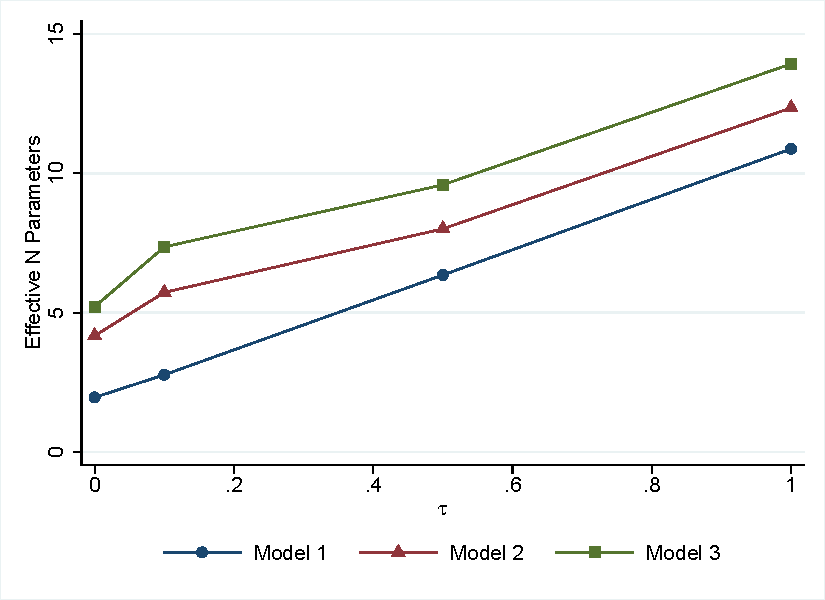
\includegraphics[height=3in, trim = 1mm 1mm 1mm 1mm, clip=true]
	{chapter_2/figs/p_newitems.pdf}
	\caption{Estimated effective number of parameters for models fit to test data consisting of the same persons responding to new items.}
	\label{fig:k-new-items}
\end{figure}

\begin{figure}[tbp]
	\centering
	\includegraphics[height=3.5in, trim = 1mm 1mm 1mm 1mm, clip=true]
	{chapter_2/figs/select_aic2.pdf}
	\caption{Proportion of times each model was selected using AIC with the ``inverted'' models.}
	\label{fig:select-aicitem}
\end{figure}




\newpage
\chapter{Bayesian cross-validation with the doubly explanatory model}
\chaptermark{Bayesian cross-validation}
The final chapter takes advantage of the Bayesian framework to implement effective (I expect) methods for the selection of item covariates. 
With MCMC methods, the doubly explanatory model may be estimated maintaining both the person and item residuals, and recently developed Bayesian cross-validation approximations are readily calculated from the conditional likelihood given these residuals after MCMC simulation. 
However, these approximations correspond to a cross-validation scheme in which holdout data include new responses from the same persons and same items. 
For inferences requiring, for example, cross-validation over items, I will show that a marginal variation of these approximations is superior (I expect).
The methods are first introduced for a simpler model and are then extend to the doubly explanatory model.


\section{WAIC and Bayesian LOO}

As a simple example, consider a hierarchical model (not cross-clustered) in which a response $y_{jk}$ has a likelihood, 
$p(y_{jk} | \theta_k)$, 
that is conditional on a cluster-specific parameter $\theta_k$. This parameter has a hierarchical prior,
$\theta_k \sim \mathrm{N}(0, \psi)$, and in turn the variance has as a prior
$\psi \sim \mathrm{log~N}(0, 1)$, an arbitrary choice. For Bayesian cross-validation, the pointwise predictive density is defined as the conditional likelihood integrated over the posterior distributions of all parameters. For the simple example, this quantity is
\begin{equation} 
	\mathrm{PD}_{jk} = 
	\iint
		p(y_{jk} | \theta_k)
		p(\theta_k | D, \psi)
		p(\psi | D)
	~d \theta_k d \psi
,\end{equation}
where $D$ represents all the data, in this case merely the complete response vector.
The log of $\mathrm{PD}_{jk}$ may be summed across observations to calculate a full data log-likelihood.
In an MCMC simulation with $S$ posterior draws, this quantity may be evaluated at each posterior draw $s$ as
\begin{equation} 
	\mathrm{PD}_{jk}^{(s)} = 
	p(y_{jk} | \theta_k^{(s)})
	p(\theta_k^{(s)} | D, \psi^{(s)})
	p(\psi^{(s)} | D)
,\end{equation}
where $\theta_k^{(s)}$ represents the posterior draw of $\theta_k$ at MCMC iteration $s$ and likewise for $\psi^{(s)}$.
$\mathrm{PD}_{jk}^{(s)}$ may be aggregated across draws to estimate the posterior distribution of $\mathrm{PD}_{jk}$. Usually this topic is discussed in terms of the \emph{log} pointwise predictive density (for example, \cite{gelman2014understanding}), but breaking from this norm simplifies some notation that follows.

Keeping with the simple example, WAIC \parencite{watanabe2010asymptotic}, a Bayesian information criteria, is defined as
\begin{equation} \label{eq:waic}
	\mathrm{WAIC} = 
		\sum_{k=1}^K \sum_{j=1}^J \log  
			\left (\frac{1}{S} \sum_{s=1}^{S} \mathrm{PD}_{jk}^{(s)} \right ) -
		\sum_{k=1}^K \sum_{j=1}^J V_{s=1}^{S} 
			\left ( \log \mathrm{PD}_{jk}^{(s)} \right )
\end{equation}
where $V_{s=1}^{S}$ represents the sample variance.
Like other information criteria, it has the form of log likelihood minus a penalty term. The penalty term for WAIC is estimated from the variances of the log pointwise predictive densities. Although the equation shows separate summations over $j$ and $k$, the summations are only a means of aggregating over the full data and do not really reflect the nested nature of the data. WAIC bears some similarity to DIC \parencite{Spiegelhalter2002} but is more stable \parencite{vehtari2015efficient}.

Bayesian LOO is an estimate of the $\mathrm{PD}_{jk}$ that would result from leave one out cross-validation. 
\textcite{gelfand1992model} propose estimating this quantity using importance sampling, and \textcite{vehtari2015efficient} propose smoothing the distribution of importance weights by fitting a generalized Pareto distribution to the upper tail of the weights.


\section{Marginal forms of WAIC and Bayesian LOO}

A limitation of cross-validation approximations relying on $\mathrm{PD}_{jk}^{(s)}$ is that they imply a cross-validation scheme in which the same clusters are represented in the holdout dataset. For inferences regarding cross-validation with new clusters, I propose a marginal predictive pointwise density:
\begin{equation} \label{eq:mpd-easy}
	\mathrm{MPD}_{k}^{(s)} = 
	%\log 
	\left (
		\left [ \int
			p(\check \theta | \psi^{(s)})
			\prod_{j} p(y_{jk} | \check \theta)
			~d \check \theta
    \right ]
		p(\psi^{(s)} | D)
	\right )
.\end{equation}
The accent is placed on $\check \theta$ to indicate that it is not 
drawn from its posterior distribution but from its ``prior'' distribution, given the posterior draw of $\psi^{(s)}$. 
In short, the bracketed quantity is the joint likelihood of cluster $k$ integrated over $p(\check \theta | \psi^{(s)})$, which is not directly influenced by data from cluster $k$.
This is similar to marginalizing over ``random effects'' in frequentist mixed models, except here it occurs at every posterior draw $s$. $\mathrm{MPD}_{k}^{(s)}$ may be used in place of $\mathrm{PD}_{jk}$ for calculating WAIC and Bayesian LOO when cross-validation with clusters is needed. The integration in Equation~\ref{eq:mpd-easy} has a closed form for linear models, and for models with non-linear link functions I proposed estimating it with adaptive quadrature \parencite{naylor1982applications}, which has been shown to work well for models with discrete outcomes and large clusters \parencite{rabe2005maximum}.

Returning now to the context of the doubly explanatory model, the pointwise predictive density is
\begin{equation} \label{eq:eirm-lpd}
	\mathrm{PD}_{ip}^{(s)} = 
		p(y_{ip} | \zeta_p^{(s)}, \epsilon_i^{(s)})
		p(\zeta_p^{(s)} | D, \sigma^{(s)})
		p(\epsilon_i^{(s)} | D, \tau^{(s)}) 
		p(\sigma^{(s)}, \tau^{(s)} | D)
,\end{equation}
where $D$ again represents all the data, in this case including all responses in $y$, the person covariate matrix $W$, and the item covariate matrix $X$. For models for cross-clustered data, including the doubly explanatory model, I propose calculating the marginal pointwise predictive density in such a way as to be marginal in regard to one set of clusters but not the other. For cross-validation over persons,
\begin{equation}
	\mathrm{MPD}_p^{(s)} = 
		\left [ \int
			p(\check \zeta | \sigma^{(s)})
			\prod_{i=1}^I	p(y_{ip} | \check \zeta, \epsilon_i^{(s)})
			~d \check \zeta 
		\right ]
		p(\epsilon^{(s)} | D, \tau^{(s)}) 
		p(\sigma^{(s)}, \tau^{(s)} | D)
\end{equation}
is appropriate. Here it is assumed that the same items would be administered to new person, and so the quantity is marginal only in regards to persons. On the other hand,
\begin{equation}
	\mathrm{MPD}_i^{(s)} = 
		\left [ \int
			p(\check \epsilon | \tau^{(s)})
			\prod_{p=1}^P	p(y_{ip} | \zeta^{(s)}, \check \epsilon_i)
			~d \check \epsilon 
		\right ]
		p(\zeta^{(s)} | D, \sigma^{(s)}) 
		p(\sigma^{(s)}, \tau^{(s)} | D)
,\end{equation}
which is marginal in regards to items, may be used for cross-validation over items.


\section{Simulation study 1: Linear responses}

I will conduct a simulation study, similar to those in Chapter~2, that evaluates the success that standard and marginal versions of WAIC and Bayesian LOO exhibit in selecting the correct model among models with differing item covariates. I will first use a version of the doubly descriptive model that is modified to have a continuous response variable. Doing so will allow me simultaneously study (1) how WAIC and Bayesian LOO perform when the likelihoods need not be approximated and (2) the accuracy of adaptive quadrature as compared against the exact likelihoods.

Owing to the relative slowness of MCMC simulation, this simulation study will involve fewer conditions as compared to those in Chapter~2 and may not incorporate holdout cross-validation. Also, if simulation study~2 (below) is highly successful, simulation study~1 may be abbreviated or omitted. Preliminary results indicate that adaptive quadrature works very well in simpler random intercept models. Also for the random intercept model, I find that the marginal forms of WAIC and Bayesian LOO are successful in choosing the generating model in a high proportion of replications.


\section{Simulation study 2: Categorical responses}

The second simulation study will use the unmodified doubly explanatory model. It will track the success that standard and marginal versions of WAIC and Bayesian LOO exhibit in selecting the correct model among models with differing item covariates. It will be very similar to simulation study~1, with the only difference being the binary response variable and the use of adaptive quadrature.


% \appendix
% \chapter{More Monticello Candidates}

\printbibliography

\end{document}
